\documentclass[border=6pt]{standalone}
\usepackage{amsmath}
\usepackage{tikz}
\usetikzlibrary{arrows.meta}
\begin{document}
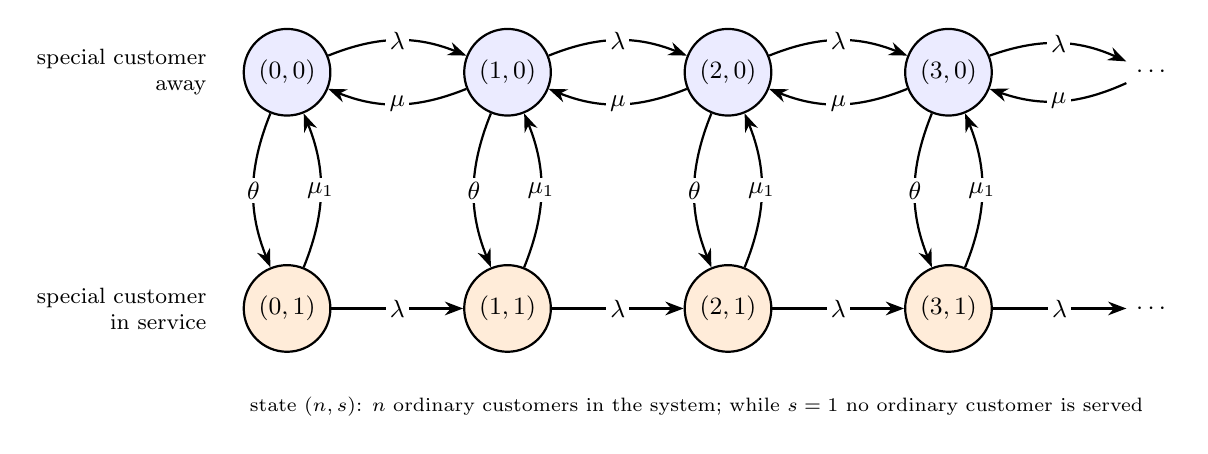
\begin{tikzpicture}[>=Stealth,font=\small,
 s/.style={draw,thick,circle,minimum size=1.1cm,inner sep=0pt,fill=blue!8},
 e/.style={->,thick},
 lab/.style={font=\small,fill=white,inner sep=1.5pt},
 every loop/.style={->,thick,looseness=6}]
\foreach \x/\n in {0/0,2.8/1,5.6/2,8.4/3} {
  \node[s] (a\n) at (\x,0) {$(\n,0)$};
  \node[s,fill=orange!15] (b\n) at (\x,-3) {$(\n,1)$};
  \draw[e] (a\n) to[bend right=22] node[lab]{$\theta$} (b\n);
  \draw[e] (b\n) to[bend right=22] node[lab]{$\mu_1$} (a\n);
}
\node (ad) at (11,0) {$\cdots$};
\node (bd) at (11,-3) {$\cdots$};
\foreach \a/\b in {0/1,1/2,2/3,3/d} {
  \draw[e] (a\a) to[bend left=22] node[lab]{$\lambda$} (a\b);
  \draw[e] (a\b) to[bend left=22] node[lab]{$\mu$} (a\a);
  \draw[e] (b\a) -- node[lab]{$\lambda$} (b\b);
}
\node[font=\footnotesize,anchor=east,align=right] at (-0.9,0) {special customer\\away};
\node[font=\footnotesize,anchor=east,align=right] at (-0.9,-3) {special customer\\in service};
\node[font=\scriptsize,align=center] at (5.2,-4.25) {state $(n,s)$: $n$ ordinary customers in the system; while $s=1$ no ordinary customer is served};
\end{tikzpicture}
\end{document}
